\section{Laufzeitsicht}
\subsection{Templates anlegen}
Author: Nha-Dan Tran\\
Um Templates für verschiedene Objekte zu generieren, verwendet die JavaFX-Anwendung ein Factory Pattern. Der Ablauf beginnt, wenn der Benutzer auf einen speziellen Button klickt. Das Ereignis wird von der JavaFX-Anwendung verarbeitet, indem sie einen ButtonHandler aufruft. Der ButtonHandler ist für die Handhabung von Benutzeraktionen zuständig und initiiert die Erstellung von Templates durch die Factory.

Die Factory wird angewiesen, ein Brett-Template zu erstellen. Dazu ruft der ButtonHandler die entsprechende Methode in der Factory auf (createTemplate("Brett")). Die Factory instantiiert daraufhin ein Brett-Template und gibt diese Instanz zurück. Dieselbe Prozedur wird für Paket- und Stütze-Templates wiederholt. Der ButtonHandler koordiniert die Erstellung der Templates für jedes spezifizierte Objekt durch Aufrufen der entsprechenden Methoden in der Factory.

Das Factory Pattern ermöglicht es der Anwendung, flexibel und dynamisch Templates zu erstellen, ohne an die konkreten Klassen der Templates gebunden zu sein. Dies fördert die Wartbarkeit und Erweiterbarkeit des Systems, da neue Templates einfach hinzugefügt werden können, ohne die bestehende Logik zu ändern.

Dieser Prozess gewährleistet, dass die JavaFX-Anwendung effizient und klar strukturiert bleibt, indem sie die Erstellung von Templates auf eine abstrahierte Factory-Schnittstelle delegiert, die für die Auswahl und Erzeugung der richtigen Templates verantwortlich ist.


\begin{figure}[H]
    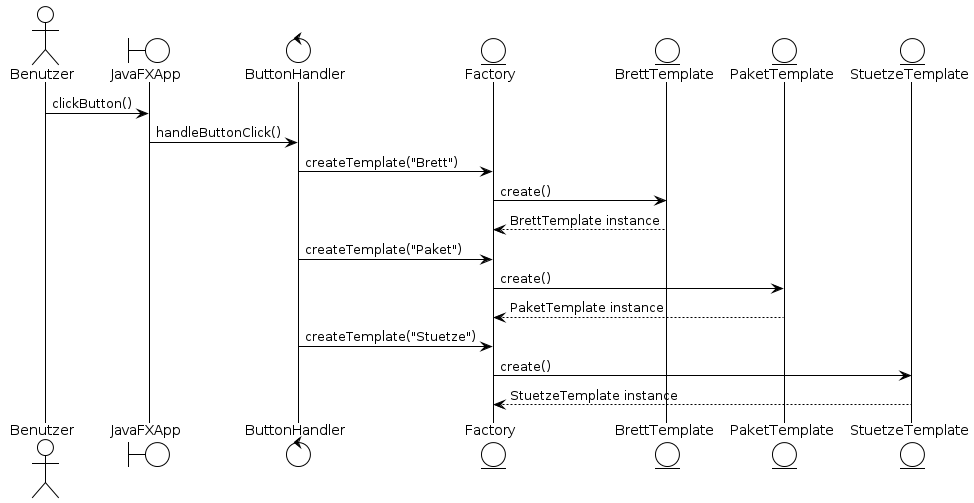
\includegraphics[width=\linewidth]{images/laufzeitsicht/laufzeitsichtTemplates.png}
    \label{fig:templateLaufzeit}
    \captionbelow{Fachlicher Kontext}
\end{figure}

\subsection{Pakete verschieben}
Author: Aron-Merlin Schlegel\\
Das Sequenzdiagramm zeigt den detaillierten Ablauf, der ausgelöst wird, wenn ein Benutzer ein Paket innerhalb der GUI verschiebt und loslässt. Diese Aktion wird durch den Benutzer initiiert und durchläuft mehrere Schritte, bis die neue Position des Pakets validiert und gegebenenfalls die GUI aktualisiert wird.

Der Prozess beginnt damit, dass der Benutzer das Paket mit der Maus auswählt und verschiebt (`onMousePressed` und `onMouseDragged`). Diese Ereignisse werden von der `PaketComponent` erfasst und an den `RegalTeilController` weitergeleitet. Der `RegalTeilController` speichert die Anfangsposition des Pakets, um bei Bedarf später darauf zurückgreifen zu können. Während der Drag-Phase wird das visuelle Feedback durch Translation des Pakets angepasst.

Beim Loslassen der Maus (`onMouseReleased`) initiiert der `RegalTeilController` die Validierung der neuen Position des Pakets. Diese Validierung wird durch den `ValidationService` durchgeführt, der die Methode `checkPlacement` aufruft. Hierbei wird geprüft, ob die neue Position des Pakets mit anderen Objekten kollidiert oder toleriert werden kann. Falls eine Kollision erkannt wird, wird die Position des Pakets zurückgesetzt und der `ErrorHandler` wird aufgerufen, um eine entsprechende Fehlermeldung in der `FehlermeldungView` anzuzeigen.

Wenn keine Kollision oder Intoleranz festgestellt wird, aktualisiert der `RegalTeilController` die Position im `PaketModel` mit den Methoden `setXPos` und `setYPos`. Das `PaketModel` informiert dann alle registrierten Observer, wie die `RegalTeilView`, über die neuen Positionen des Pakets, wodurch die Anzeige automatisch aktualisiert wird.

\begin{figure}[H]
    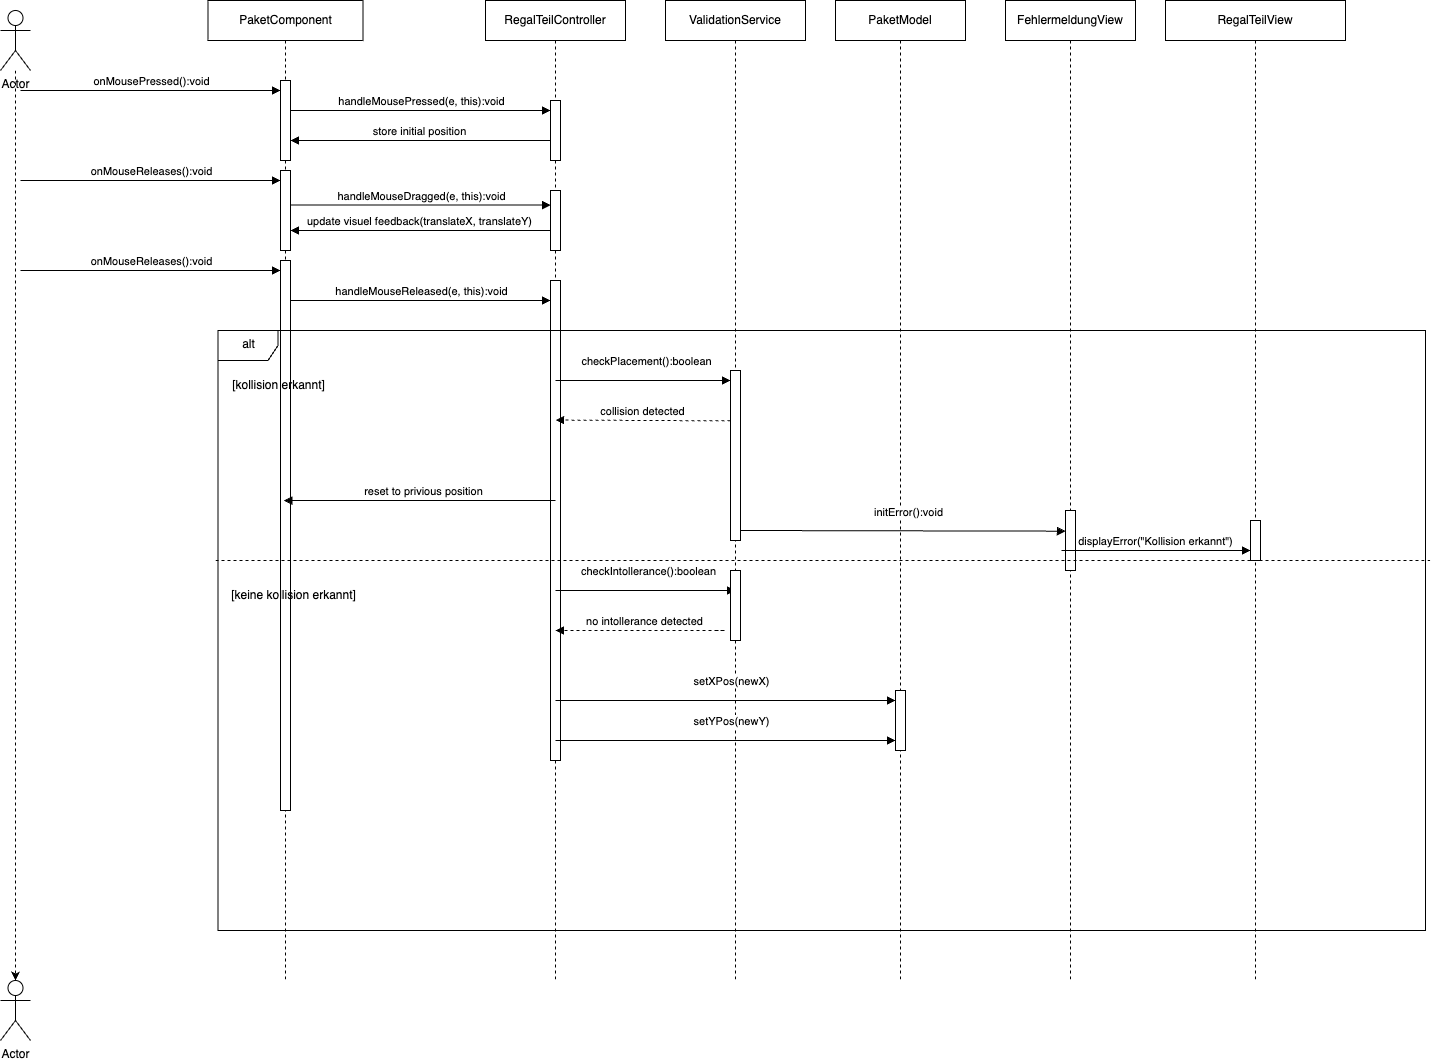
\includegraphics[width=\linewidth]{images/laufzeitsicht/SequenzdiagrammPaketVerschieben.drawio.png}
    \label{fig:PaketVerschiebenLaufzeit}
    \captionbelow{Fachlicher Kontext}
\end{figure}

\subsection{Sequenz 1: Stütze erstellen}
\begin{figure}[H]
    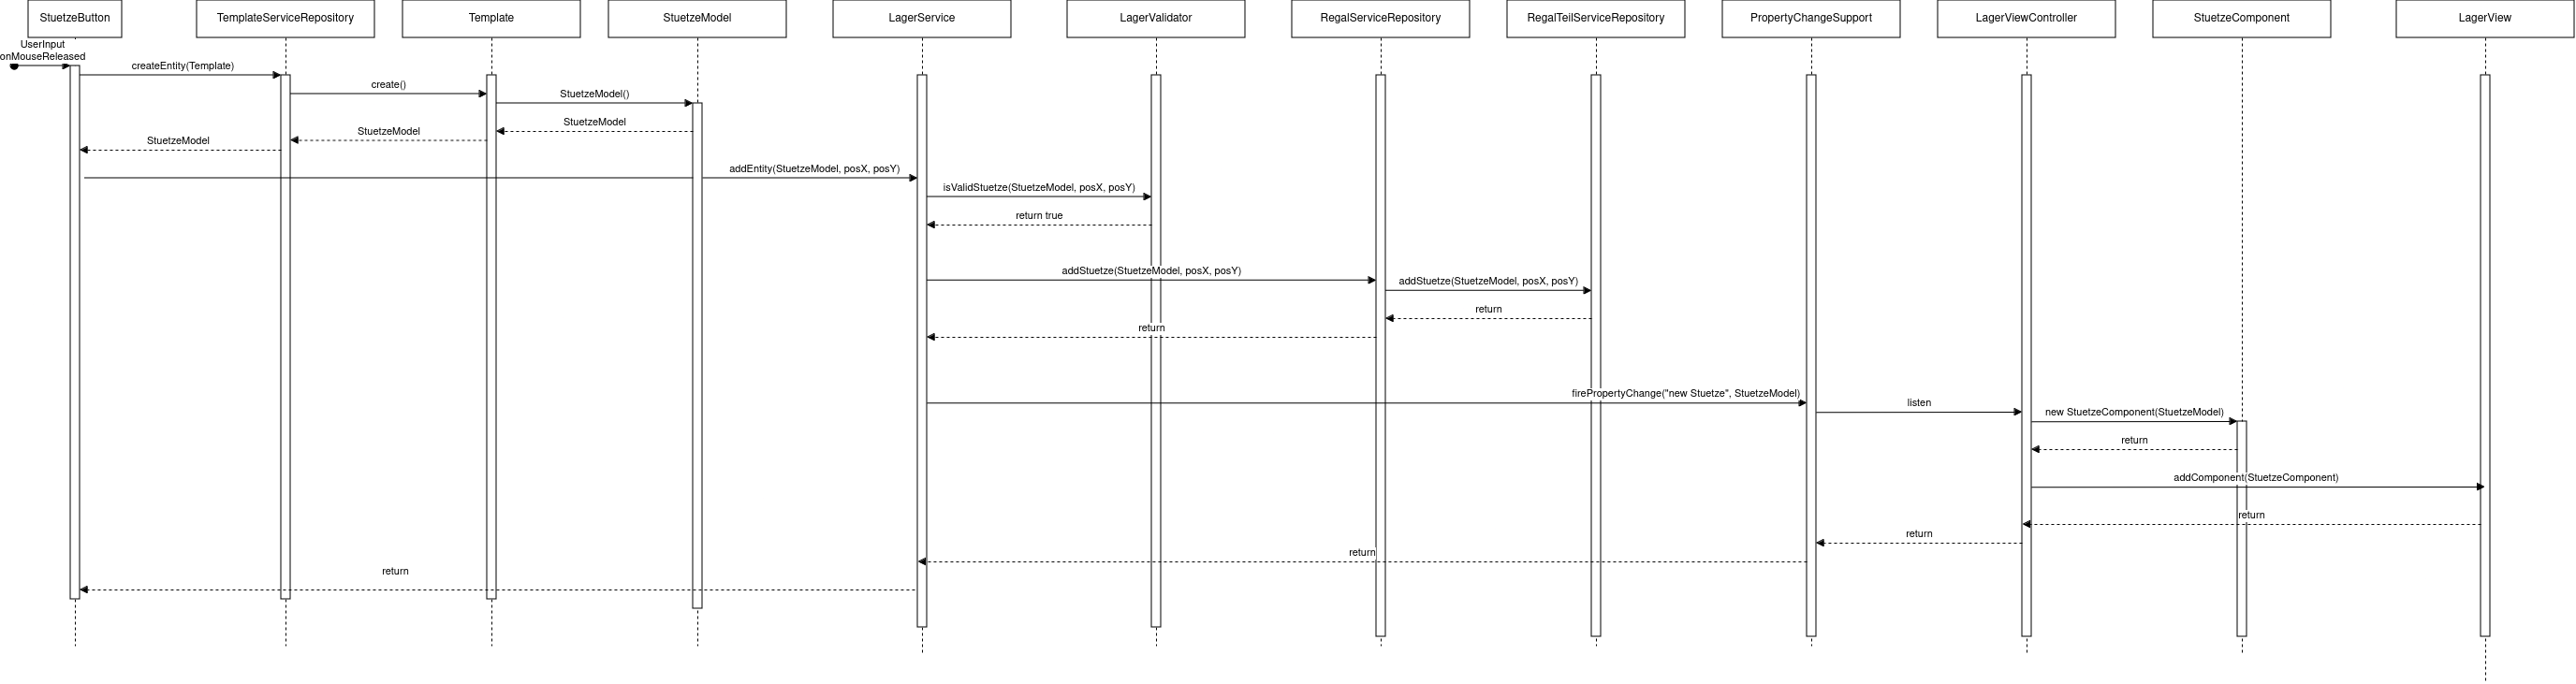
\includegraphics[width=\linewidth]{images/laufzeitsicht/Sequenz_David.png}
    \captionbelow{Sequenzdiagramm: Stütze erstellen}
    \label{fig:Sequenzdiagramm1}
\end{figure}
Durch das MausReleased Event ruft der TemplateButton zuerst den TemplateService auf, wodurch ein StuetzeModel erzeugt wird. Der Button reicht dieses Model, zusammen mit den Koordinaten des Mausevents dann an den LagerService weiter, um die Platzierung anzustoßen. Der LagerService lasst den Validator prüfen, ob die Stütze an dieser Position platziert werden kann - in diesem Fall ist das möglich. Danach baut der LagerService die Stütze ins Modell ein (mit den jeweiligen Subservices) und feuert eine Änderungen an den PropertyChangeSupport. Dieser informiert seine Listener, in diesem Fall der LagerViewController, welcher eine neue StuetzeComponent erzeugt und in den Graphen des LagerView einhängt.